\section{Previous work}

Light transport in participating media is governed by the radiative transfer equation~(RTE), first studied in the context of astrophysics by Chandrashekar~\cite{Chandrasekhar60} and later used for rendering in graphics by Kajiya~\cite{Kajiya86}. Today, this equation is typically solved using Monte Carlo based methods. However, in strongly scattering media or in the presence of highly anisotropic phase functions, these methods can become prohibitive, due to the high computational cost, which comes from tracing long particle paths with many scattering events.

In contrast to path-tracing, the $P_N$-method is a deterministic method, which gives a solution by solving a system of linear equations. It is derived by discretizing the angular variable of the radiative transfer equation into spherical harmonics (SH). This gives rise to a set of coupled, complex-valued partial differential equations, called $P_N$-equations. The subscript $N$ refers to the truncation order of the SH. 

The $P_N$-method has a long history in other fields and was never applied in graphics. Kajia~\cite{Kajiya84} explained the theory, but did not give any details on implementation or how to solve it. In fact, as Max~\cite{Max95} pointed out, it is not clear if Kajiya succeeded at all at applying the method, as all of the results in his paper were produced with a simpler method. This is further strengthened by our observation, that a straight forward finite difference discretization of the $P_N$-equations produces unuseable results, due to oscillation artifacts in the solution. In our paper, we derive the real-valued $P_N$-equations along with a staggered-grid solver, that produces artifact free solutions.

\begin{figure}[h]
\centering
\begin{subfigure}{0.45\columnwidth}
%\missingfigure{test}
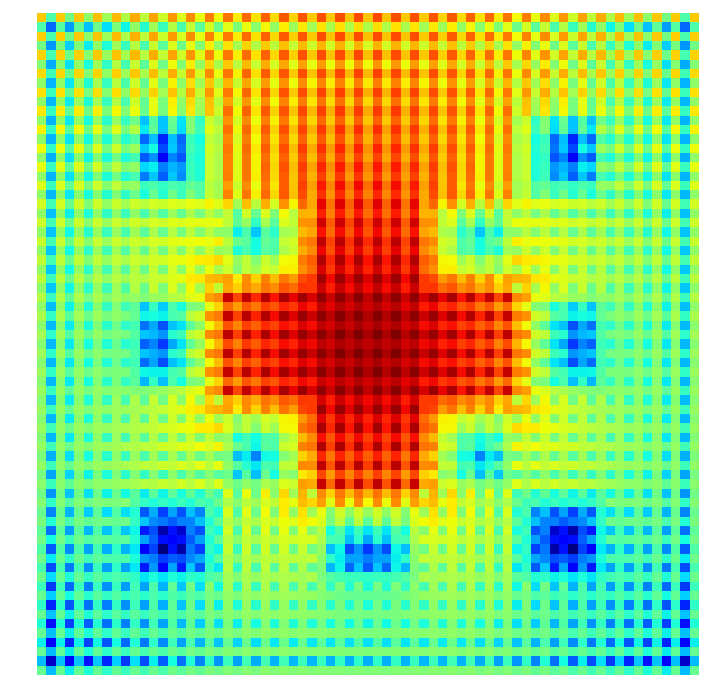
\includegraphics[width=\columnwidth]{images/checkerboard2d_p1_collocated.png}
\end{subfigure}%
\hspace{0.05\columnwidth}
\begin{subfigure}{0.45\columnwidth}
%\missingfigure{test2}
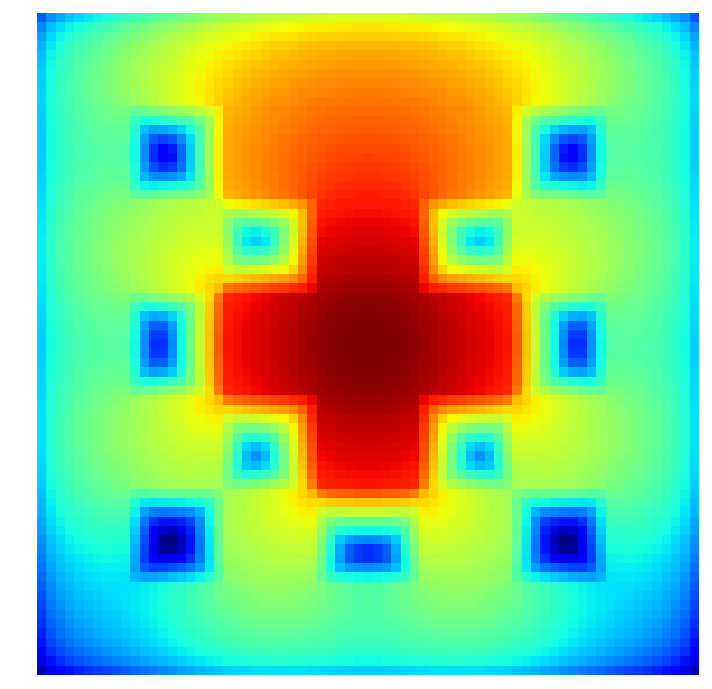
\includegraphics[width=\columnwidth]{images/checkerboard2d_p1_staggered.png}
\end{subfigure}%
\vspace{-0.1in}
\icaption{Solving the 2D-checkerboard problem using naive collocated grids produces oscillating artefacts (left). Our solver uses staggered grids and produces artefact free results (right).}
\label{fig:artifacts}
\end{figure}


Similar to $P_N$, the classical diffusion approximation (CDA) is a deterministic method, which arrives at a solution by solving a system of linear equations. It is derived as a degenerate case of the $P_1$-equations (truncation after the first SH order), which collapses to a simple diffusion equation giving the method its name. CDA has a long history in other domains, such as astrophysics~\cite{Ishimaru78} and was introduced to graphics by Stam \cite{Stam95}. It was further extended to anisotropic radiative transfer by \cite{Jakob10}.

CDA suffers from severe energy loss close to regions with strong density gradients. The problem is addressed by a modification known as Variable Eddington factor (VEF), which nonlinearly adjusts the diffusion coefficient to improve the solution near density gradients and low-density regions. Flux-limited diffusion, developed in the context of astrophysics by Levermore et al.~\cite{Levermore81} and later introduced to graphics by Koerner et al.~\cite{Koerner14}, is the most prominent example.

The idea behind VEF is to derive a better diffusion coefficient by seeing it as a mean to spatially blend between the diffusive and pure transport regime. The diffusive regime is where thick highly scattering media is present and causes photons to change directions in short succession, while the transport regime in thin and highly absorbing media causes photons to travel long straight lines. In the absence of scattering (e.g. pure vacuum), the non-linear diffusion coefficient turns the diffusion equation into an advection equation.

It is an open and unresolved question, whether the $P_N$-method with truncation at higher order, gives any benefit over using first order non-linear diffusion. It is also been raised in other domains~\cite{Olson00} and resolving it is one motivation for this paper.
 
%\begin{itemize}
  %\item Alternative deterministic methods
  %\begin{itemize}
  %  \item Heuristics \cite{Kaplanyan10} \cite{Elek14}
  %  \item Lattice Boltzmann Methods \cite{Geist04}
  %  \item Discrete Ordinates \cite{Languenou95}
  %\end{itemize}
  %However, among all the deterministic methods, the diffusion approximation has been the most popular due to its intuition and simplicity.


%\end{itemize}

